\chapter{\acrlong{av}}
\section{Allgemeines}
Ein \acrfull{av} ist der erste Verteidigungsmechanismus in einem Netzwerk. Angriffe, darunter Schadsoftware, kommen in den meisten Fällen über einen Endpoint (z.B. Notebook) in ein Firmennetzwerk.\\

Eine gegebene Struktur ist immer nur so stabil, wie sein schwächstes Glied. Dies gilt bei Häusern wie auch bei Computernetzwerken.
Oftmals ist das schwächste Glied ein Client oder ein Server, da diese Geräte vielfach mit dem Internet kommunizieren.
Dies macht genau diese Geräte besonders schützenswert.\\

Server und Clients werden mit einem \acrlong{av} versucht zu schützen. Ein Antivirus hilft bekannte Schadsoftware zu detektieren und zu entfernen.
Neue Schadsoftware wird versucht mit komplexen Algorithmen zu erkennen und deren Vorhaben zu blockieren.
Schadsoftware kann sich sehr schnell vermehren und sich im ganzen Netzwerk ausbreiten. 
Das kann den Effekt haben, dass die ganze Unternehmung beeinträchtigt wird.
Deshalb ist eines der wichtigesten Erkenntnisse, dass ein \acrlong{av} auf \textbf{allen} Endpoints (Server und Client) benötigt wird.





\section{Windows Defender}
\acrfull{av} Programme kommen in allen Arten und Formen.
Es ist schwer den Überblick über die Landschaft der \acrlong{av} Programme zu behalten.\\


Microsoft bietet für seine Produkte einen eigenen kostenfreien \acrlong{av} an.
Der Windows Defender ist nicht eine allround Lösung, wie andere \acrshort{av} Produkte, mit unzähligen Features.
Er ist einer der besten kostenfreien Lösungen und ist für KMUs sehr geeignet, da dort meist keine massgeschneiderte Lösung gewünscht wird.
Laut dem \href{https://www.microsoft.com/security/blog/2021/05/11/gartner-names-microsoft-a-leader-in-the-2021-endpoint-protection-platforms-magic-quadrant/}{Gartner Magic Quadrant für Endpoint Protection}\footnote{Link: \href{https://www.microsoft.com/security/blog/2021/05/11/gartner-names-microsoft-a-leader-in-the-2021-endpoint-protection-platforms-magic-quadrant/}{https://www.microsoft.com/security/blog/2021/05/11/gartner-names-microsoft-a-leader-in-the-2021-endpoint-protection-platforms-magic-quadrant/}} ist die Microsoft Lösung eine der Marktführer in diesem Bereich.
Der Windows Defender erkennt die meisten Gefahren und löst die erkannten Probleme sehr kompetent.\\

\newpage

Hier eine Übersicht der Vor- und Nachteile:\\

\begin{minipage}{\linewidth}
    \begin{multicols}{2}
        \begin{table}[H]
            \begin{center}
                \textbf{Vorteile:}
                \begin{itemize}
                    \item kostenfrei
                    \item Realtime Protection funktioniert zuverlässig
                    \item in Windows integriert
                    \item einfache Bedienung
                \end{itemize}
            \end{center}
            \caption{Vorteile Windows Defender}
        \end{table}
        \begin{table}[H]
            \begin{center}
                \textbf{Nachteile:}
                \begin{itemize}
                    \item beschränkte Konfigurationsmöglichkeiten
                    \item Keine cloudbasiertes Dashboard/Management
                    \item Machine Learning nicht vorhanden
                \end{itemize}
            \end{center}
            \caption{Nachteile Windows Defender}
        \end{table}
    \end{multicols}
\end{minipage}


\subsection{Wazuh Integration}
In Wazuh existieren Regeln, welche das Verhalten vom Windows Defender loggen.
Dazu gehören auch alle durchgeführten Scans.\\

Die wichtigsten zwei Regeln sind folgende:
\subsubsection{Real-time protection disabled}
Wenn die Real-time Protection deaktiviert wird, kann möglicherweise bösartige Software ausgeführt werden.
Daher wird in Wazuh ein Level 12 Alert erstellt: 

\begin{figure}[H]
    \centering
    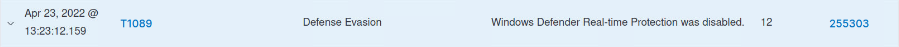
\includegraphics[width=\linewidth]{../img/AV/real-time-protection.png}
    \caption{Real-time Protection wurde deaktiviert}
\end{figure}


\subsubsection{Defender found a threat}
Wenn schädliche Software auf einen Computer herunterdeladen wird, sollte Windows Defender diese erkennen.
Somit wird folgender Alert generiert:
\begin{figure}[H]
    \centering
    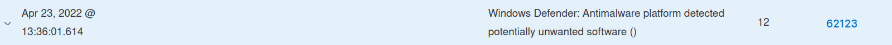
\includegraphics[width=\linewidth]{../img/AV/defender-detection.png}
    \caption{Malware wurde entdeckt}
\end{figure}

Auf diesen Alert sollte normalerweise folgender Alert folgen:
\begin{figure}[H]
    \centering
    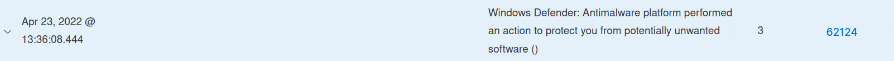
\includegraphics[width=\linewidth]{../img/AV/defender-removal.png}
    \caption{Malware wurde entfernt}
\end{figure}

Dieser bestätigt, dass Windows Defender die schädliche Software entfernt hat.